\subsection{Petalinux}
\label{subsec:embedded_platform:operating_systems:petalinux}

% built with petalinux tools
Xilinx provides Petalinux tools to build your own Petalinux operating system.
It is recommended to work with the so called target platform.
The target platform is a combination of hardware and software components.
The most important hardware component is a proprietary file format, called XSA.
XSA stands for Xilinx Support Archive and contains one or more hwh files, bit files, driver files and other meta-data files.
In a hardware hand-off file (hwh file), information about Vivado tool version and the board tag are saved.
Furthermore, hwh files contain IP-instance, name and parameters, as well as Memory Map information of the processors \cite{vitis_user_guide}.

It is also possible to download the pre-built platform from Element14.
However, to customize the working environment, it is needed to build the platform by hand.
Avnet provides all files for the Ultra96-V2 board via Github to build an own target platform.

\paragraph{Development Flow}
Graphic \ref{fig:petalinux_workflow} shows the working flow graphically.
Each of the blocks is described in the following sections.

\begin{figure}[h]
	\centering
	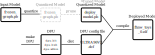
\includegraphics[width=1\textwidth]{graphics/workflow.pdf}
	\caption{Petalinux workflow}
	\label{fig:petalinux_workflow}
\end{figure}

\paragraph{Build own Vitis Platform}
Four repositories are needed from Avnet.
\begin{itemize}
	\item \texttt{bdf}
	\item \texttt{hdl}
	\item \texttt{petalinux}
	\item \texttt{vitis}
\end{itemize}

The \texttt{bdf} (board definition files) repository contains one folder for each of their development boards.
The \texttt{hdl} repo is needed to use the programmable logic on UltraScale+ MPsoC.
In the \texttt{petalinux} archive are, among other things, the configurations of the Petalinux operating system.
To be able to build a Vitis platform, the \texttt{vits} archive is needed as well.
The \texttt{vitis} folder contains several makefiles which refer to the other three repositories.
The repositories \texttt{hdl} and \texttt{petalinux} need to be checked out on the same branch as the Xilinx tools are.

The building process can be started by the makefile in the vitis folder.
Which board is used, needs to be given as a parameter.
Building the platform needs several hours, approximately \SI{200}{GB} disk space and a minimum of \SI{32}{GB} RAM is required.
After the process is done, the platform is located in the platform\_repo directory.

The makefile from Avnet creates a sysroot by default.
Because all header and library files are included in this directory structure, cross compiling an application is possible.

\paragraph{Configure own Vitis Platform}
The platform can be customized according to individual needs.
First a new Petalinux project is created.
The generated folder \texttt{project-spec/meta-user} contains recipes to add or remove programs such as \acrshort{opencv} or a package manager.
Own recipes can be created by the \texttt{petalinux-create -t apps} command.
It is possible to create a component from an existing content or from a pre-defined application template \cite{petalinux_commandline_guide}.

After adding all recipes, the \texttt{petalinux-config} and \texttt{petalinux-build} command create the customized root filesystem, the boot files and the Linux kernel \cite{petalinux_user_guide}.

The first stage bootloader, the device tree blob and u-boot are stored in the \texttt{BOOT.BIN} file by default configuration.
They are needed to first initialize the board and load the kernel image \cite{xilinx_wiki_boot}.
The kernel image is in the \texttt{Image.ub} file \cite{xilinx_wiki_uboot}.
They are located in the \texttt{petalinux/projects/ultra96v2\_oob\_2019\_2/images/linux} directory.

\paragraph{Flash SD Card}
The first step is to create the partitions for the boot files and for the root filesystem.
For the boot partition, the format should be fat32, while the root filesystem partition should to be ext4.
A space of \SI{1}{GB} for the boot partition is enough.
Furthermore, the boot label should be set for the boot partition.
In a next step, the created partitions need to be formated.
In a shell script, it can be done like this:

\begin{lstlisting}[style=bash, caption={Prepair SD card}, label=lst:create_partitions]
  DISK=/dev/sdb
  PART=

  # Create partitions
  sudo parted $DISK -s mkpart primary fat32 1MiB 1025MiB
  sudo parted $DISK -s mkpart primary ext4 1026MiB 100%

  # Set boot label
  sudo parted $DISK -s set 1 boot on

  # format partitions
  sudo mkfs -t vfat -F 32 -n boot $DISK${PART}1
  sudo mkfs -t ext4 -L rootfs $DISK${PART}2
\end{lstlisting}

The SD card is now ready to save the \acrshort{os}.
The \texttt{BOOT.BIN} and \texttt{Image.ub} can be copied to the boot partition and the \texttt{rootfs.tar.gz} extracted to the rootfs partition.

\paragraph{Setup}
\todo[inline]{all}